\documentclass[12pt,letter]{article}

% Packages
\usepackage[utf8]{inputenc}
\usepackage{graphicx}
\usepackage{geometry}
\geometry{margin=1in}
\usepackage{hyperref}
\usepackage{amsmath}
\usepackage{booktabs}
\usepackage{listings}
\usepackage{array}
\usepackage{caption}
\usepackage{tocbibind}
\usepackage{fancyhdr}
\usepackage{setspace}
\usepackage{listings}
\usepackage{xcolor}

\lstdefinestyle{matlabstyle}{
    language=Matlab,
    backgroundcolor=\color{gray!10},   % Light gray background
    basicstyle=\ttfamily\footnotesize, % Use monospaced font
    keywordstyle=\color{blue},         % Keywords in blue
    commentstyle=\color{green!50!black}, % Comments in green
    stringstyle=\color{orange},        % Strings in orange
    numberstyle=\tiny\color{gray},     % Line numbers in gray
    numbers=left,                      % Line numbers on the left
    numbersep=5pt,                     % Space between line numbers and code
    frame=single,                      % Frame around the code
    breaklines=true,                   % Automatic line breaking
    breakatwhitespace=true,            % Break at whitespaces
    tabsize=4,                         % Size of tabs
    showspaces=false,                  % Don't show spaces
    showstringspaces=false,            % Don't show string spaces
    captionpos=b,                      % Caption position at bottom
}
\lstset{style=matlabstyle}




\title{Characterization Report: Antenna Subsystem}
\author{J.C. Vaught}
\date{Nov. 20, 2024}


% Document
\begin{document}

\maketitle
% 1. Introduction
\vfill
\section*{Introduction}

The Global Positioning System (GPS) L1 frequency band at 1575.42 MHz is pivotal for navigation and positioning applications globally. Accurate characterization of GPS antennas is essential to ensure optimal performance in signal reception and processing. This report documents the process of characterizing a GPS L1 Band active antenna, including the challenges faced due to equipment limitations and initial misunderstandings of the antenna's operational requirements.

As a non-expert venturing into RF antenna characterization, several obstacles were encountered that required iterative problem-solving and learning. This report aims to provide a detailed account of the experiments conducted, the issues faced, and the solutions implemented, serving as a practical guide for similar future endeavors.

\newpage
\section*{Antenna Specifications}

In the course of this characterization study, two distinct GPS L1 band antennas were evaluated to assess their performance. The primary antenna under examination is the \textbf{Side Mounted Cable Antenna (GPS L1)}, specifically designed for high-sensitivity GPS applications. For comparative purposes, the \textbf{Bottom Mounted Cable Antenna (GPS L1)} was also tested to establish baseline performance metrics and highlight the differences in mounting configurations.

The following tables provide detailed specifications for each antenna, outlining their operational parameters, physical characteristics, and technical features. This comparative analysis facilitates a comprehensive understanding of the performance differences and suitability of each mounting type for GPS-based applications.

\begin{table}[h!]
    \centering
    \begin{tabular}{ll}
        \toprule
        \textbf{Specification} & \textbf{Side Mounted Cable Antenna (GPS L1)} \\
        \midrule
        Center Frequency & 1575.42 MHz $\pm$ 3 MHz \\
        VSWR & $\leq$ 2:1 \\
        Polarization & Right-Hand Circular Polarization (RHCP) \\
        LNA Gain (Without Cable) & 28 dB (Typical) \\
        DC Voltage & 3 V to 5 V \\
        DC Current & 7--10 mA \\
        Impedance & 50 $\Omega$ \\
        Physical Dimensions & 35 x 30 x 15 mm \\
        Weight & 60 grams \\
        Cable & 3 m RG174 \\
        Connector & SMA Male Plug \\
        Mounting & Magnetic base (Side Mounted) \\
        Housing & Black \\
        Operating Temperature & -40°C to 85°C \\
        \bottomrule
    \end{tabular}
    \caption{Specifications of the Side Mounted Cable Antenna (GPS L1)}
    \label{tab:side_mounted_antenna}
\end{table}

\begin{table}[h!]
    \centering
    \begin{tabular}{lll}
        \toprule
        \textbf{Category} & \textbf{Specification} & \textbf{Details} \\
        \midrule
        \multicolumn{3}{l}{\textbf{Antenna}} \\
        \midrule
        & Center Frequency & 1575.42 MHz $\pm$ 3 MHz \\
        & Band Width & CF $\pm$ 5 MHz \\
        & Polarization & Right-Hand Circular Polarization (RHCP) \\
        & Gain & 2 dBic (Zenith) \\
        & V.S.W.R & $\leq$ 1.5 \\
        & Impedance & 50 $\Omega$ \\
        & Axial Ratio & 3 dB (max) \\
        & Dimension & Φ46.6 × 14.5 mm \\
        \midrule
        \multicolumn{3}{l}{\textbf{LNA}} \\
        \midrule
        & Gain & 28 $\pm$ 2 dB \\
        & Noise Figure & $\leq$ 1.5 dB \\
        & Filter Insertion Loss & $\leq$ 3 dB \\
        & Ex-band Attenuation & 12 dB @ CF + 50 MHz \\
        & & 16 dB @ CF - 50 MHz \\
        & Supply Voltage & 2.2 - 5V DC \\
        & Current Consumption & $\leq$ 15 mA \\
        & V.S.W.R & $\leq$ 2.0 \\
        \midrule
        \multicolumn{3}{l}{\textbf{Mechanical}} \\
        \midrule
        & Cable & RG174, 3 meters / 9.8 feet \\
        & Connector & SMA Male \\
        & Radome Material & ABS \\
        & Mounting Method & Screw-based mount (Bottom Mounted) \\
        \midrule
        \multicolumn{3}{l}{\textbf{Environmental}} \\
        \midrule
        & Operating Temperature & -40°C ~ +85°C \\
        & Relative Humidity & Up to 95\% \\
        & Ingress Protection & IP65 ~ IP67 (excluding cable outlet) \\
        & Vibration & 10 to 55 Hz with 1.5 mm amplitude, 2 hours \\
        & Environmentally Friendly & ROHS Compliant \\
        \bottomrule
    \end{tabular}
    \caption{Detailed Specifications of the Bottom Mounted Cable Antenna (GPS L1)}
    \label{tab:bottom_mounted_antenna}
\end{table}


The \textbf{Side Mounted Cable Antenna (GPS L1)} is optimized for GPS signal reception, featuring a built-in Low Noise Amplifier (LNA) that enhances signal strength and reduces noise. Its Right-Hand Circular Polarization (RHCP) aligns with the polarization of GPS satellite signals, ensuring efficient signal capture. The active design necessitates a Bias Tee for powering the LNA, which is seamlessly integrated into the system through the SMA male plug. The magnetic base allows for secure and flexible placement on metallic surfaces, making it ideal for environments where side mounting is preferred.

In contrast, the \textbf{Bottom Mounted Cable Antenna (GPS L1)} serves as an alternative mounting configuration, offering similar performance characteristics but utilizing a screw-based mount instead of a magnetic base. This mounting method provides a more permanent installation option, suitable for fixed setups where magnetic mounting is not feasible. While both antennas share identical operational specifications, the choice between side and bottom mounting depends on the specific application requirements and environmental constraints.


\newpage
\section*{Experimental Setup}

The experimental setup for characterizing the GPS L1 Band active antennas comprised various hardware and software components, carefully selected to facilitate accurate measurements and data analysis. The primary tools included multiple Software-Defined Radios (SDRs), a Bias Tee for supplying DC power to the antenna, and computers running specialized software for signal generation and analysis.

\subsection*{Equipment Used}

\begin{table}[h!]
    \centering
    \begin{tabular}{ll}
        \toprule
        \textbf{Equipment} & \textbf{Description} \\
        \midrule
        Pluto SDR \#1 & Used for signal generation tasks. \\
        Pluto SDR \#2 & Employed for baseline comparison measurements. \\
        RTL-SDR v4 & Initially used but faced compatibility issues with MATLAB. \\
        RTL-SDR v3 & Replaced RTL-SDR v4, works with MATLAB. \\
        Bias Tee & Injects DC power into the antenna, enabling the Low Noise Amplifier. \\
        MacBook Air & Intended for controlling the SDRs; however, had compatibility issues. \\
        Windows PC & An alternative computing platform due to software issues with MacOS. \\
        SMA Cables & Used for connecting various components. \\
        USB Cables & Facilitated connections for SDRs and computers. \\
        GPS Antenna \#1 & Antenna with a side mounted cable. \\
        GPS Antenna \#2 & Antenna with a bottom mounted cable. \\
        \bottomrule
    \end{tabular}
    \caption{Hardware Components Used in Experimental Setup}
    \label{tab:equipment_used}
\end{table}


\subsection*{Software Used}

\begin{table}[h!]
    \centering
    \begin{tabular}{ll}
        \toprule
        \textbf{Software} & \textbf{Description} \\
        \midrule
        GNU Radio & Utilized for SDR control and signal processing. \\
        MATLAB & Employed for signal processing and plotting. \\
        SDR\# & Used for real-time SDR control and signal analysis. \\
        Python & Utilized for basic analysis. \\
        ChatGPT & Used for understanding problem and developing testing. \\
        \bottomrule
    \end{tabular}
    \caption{Software Components Used in Experimental Setup}
    \label{tab:software_used}
\end{table}

\subsection*{Test Environment}

Experiments were conducted in an indoor laboratory environment for Electrical Engineering Capstone Projects, thereby ensuring the integrity of the measurements. The antenna was mounted on the metallic shelves of the lab tables using its magnetic base, providing a stable and grounded setup conducive to accurate signal reception and analysis. Unfortunately, the antenna was not tested in an open outdoor area, which could have reduced multipath effects and environmental obstructions that might skew the results.

\newpage
\subsection*{Initial Challenges}

The characterization process encountered several initial setbacks that required significant troubleshooting and adjustments. The first major challenge stemmed from compatibility issues between the Pluto SDRs and the MacBook Air. Specifically, the two Pluto SDR units could not be simultaneously connected due to driver conflicts and USB bandwidth limitations, preventing concurrent signal generation and reception. This limitation necessitated a transition to using the RTL-SDR v4, which was initially believed to offer better compatibility with MATLAB and the required SDR software.

However, it was later discovered that the RTL-SDR v4 was incompatible with MATLAB due to a chipset change. This revelation necessitated the acquisition of an RTL-SDR v3, which resolved some of the compatibility issues. Despite this, many existing tutorials and resources were tailored for the RTL-SDR v4, resulting in additional time spent adapting these materials and searching through forums for relevant solutions. To facilitate signal generation and baseline testing, a Windows PC was employed alongside the MacBook Air, enabling the use of the Pluto SDRs for signal generation while leveraging the RTL-SDR v3 for reception and analysis.

Another significant hurdle was related to the antenna's power requirements. Initial tests revealed no noticeable performance difference between the GPS L1 Band active antenna and a general-purpose antenna. This lack of differentiation was traced back to the absence of a Bias Tee, which is crucial for supplying DC power to the antenna's Low Noise Amplifier (LNA). Without the Bias Tee, the LNA remained unpowered, resulting in underperformance that was mistakenly attributed to the antenna itself. This oversight led to the purchase of a Bias Tee compatible with the Pluto SDRs. Fortunately, the RTL-SDR v3 included a built-in Bias Tee capable of supplying 4.5 V, simplifying the power supply process for the active antenna.

Testing within the laboratory environment also proved suboptimal due to multipath effects, which introduced interference and distorted signal measurements. These multipath channels compromised the integrity of the received signals, highlighting the need for a more controlled or alternative testing environment to minimize such distortions. Additionally, the absence of a rotation device made it impossible to physically test the radiation pattern of the antennas, limiting this aspect of the characterization to theoretical analysis rather than empirical testing.

Furthermore, attempts to generate test signals using simple sine waves were ineffective, as these signals did not accurately replicate the complex modulation schemes characteristic of GPS signals. This resulted in unreliable measurements and underscored the necessity of developing more sophisticated signal generation techniques to emulate realistic GPS transmissions accurately. The process of configuring and calibrating the SDR software also presented a steep learning curve, requiring extensive time and effort to achieve precise and consistent measurements.



\newpage

% 4. Testing Methodology
\section*{Testing Methodology}

The characterization of the GPS L1 Band active antenna involved a series of methodical tests designed to evaluate its performance across various parameters. Each test aimed to isolate and measure specific aspects of the antenna's functionality, employing both standard and improvised techniques to overcome the challenges encountered.

\subsection*{Frequency Response}

\paragraph{Objective}
The primary objective of the frequency response test was to verify the antennas' performance across their specified frequency ranges, ensuring they operate effectively within the GPS L1 band (1575.42 MHz). This assessment is crucial for determining the antennas' suitability for high-precision GPS applications, where accurate signal reception and minimal signal distortion are paramount.

\paragraph{Procedure}
The frequency response characterization involved generating and receiving signals across a range encompassing the GPS L1 frequency. Two distinct setups were utilized, corresponding to the \textbf{Side Mounted Cable Antenna (GPS L1)} and the \textbf{Bottom Mounted Cable Antenna (GPS L1)}. The following outlines the detailed steps undertaken for each system:

\paragraph{1. Signal Generation}
For both antennas, a Pluto SDR was employed to generate a pseudo-random noise (PRN) code-modulated signal centered at 1575.42 MHz. The signal generation script was configured to sweep frequencies from 1572 MHz to 1578 MHz in 0.1 MHz increments, emulating the operational bandwidth of the GPS L1 band.

\paragraph{2. Signal Transmission}
The generated signal was transmitted through the respective antenna (side-mounted or bottom-mounted) connected to the Pluto SDR. A USB-powered Bias Tee was utilized to supply the necessary DC power to the antenna's Low Noise Amplifier (LNA), ensuring optimal signal amplification and reception.

\paragraph{3. Signal Reception}
An RTL-SDR v3 was configured to receive the transmitted signal. The received signal strength was recorded at each frequency increment to construct the frequency response profile. Due to initial compatibility issues with the RTL-SDR v4, the RTL-SDR v3 provided a reliable platform for accurate data collection.

\paragraph{4. Data Analysis}
The collected data was analyzed using MATLAB to plot the frequency response curves for both antennas. 

\paragraph{Results}

Upon completion of the frequency sweep, the received signal strength data was plotted against the swept frequencies for both the Side Mounted Cable Antenna and the Bottom Mounted Cable Antenna. The empirical results were then compared with the theoretical model to assess the antennas' performance.


\begin{figure}[h!]
    \centering
    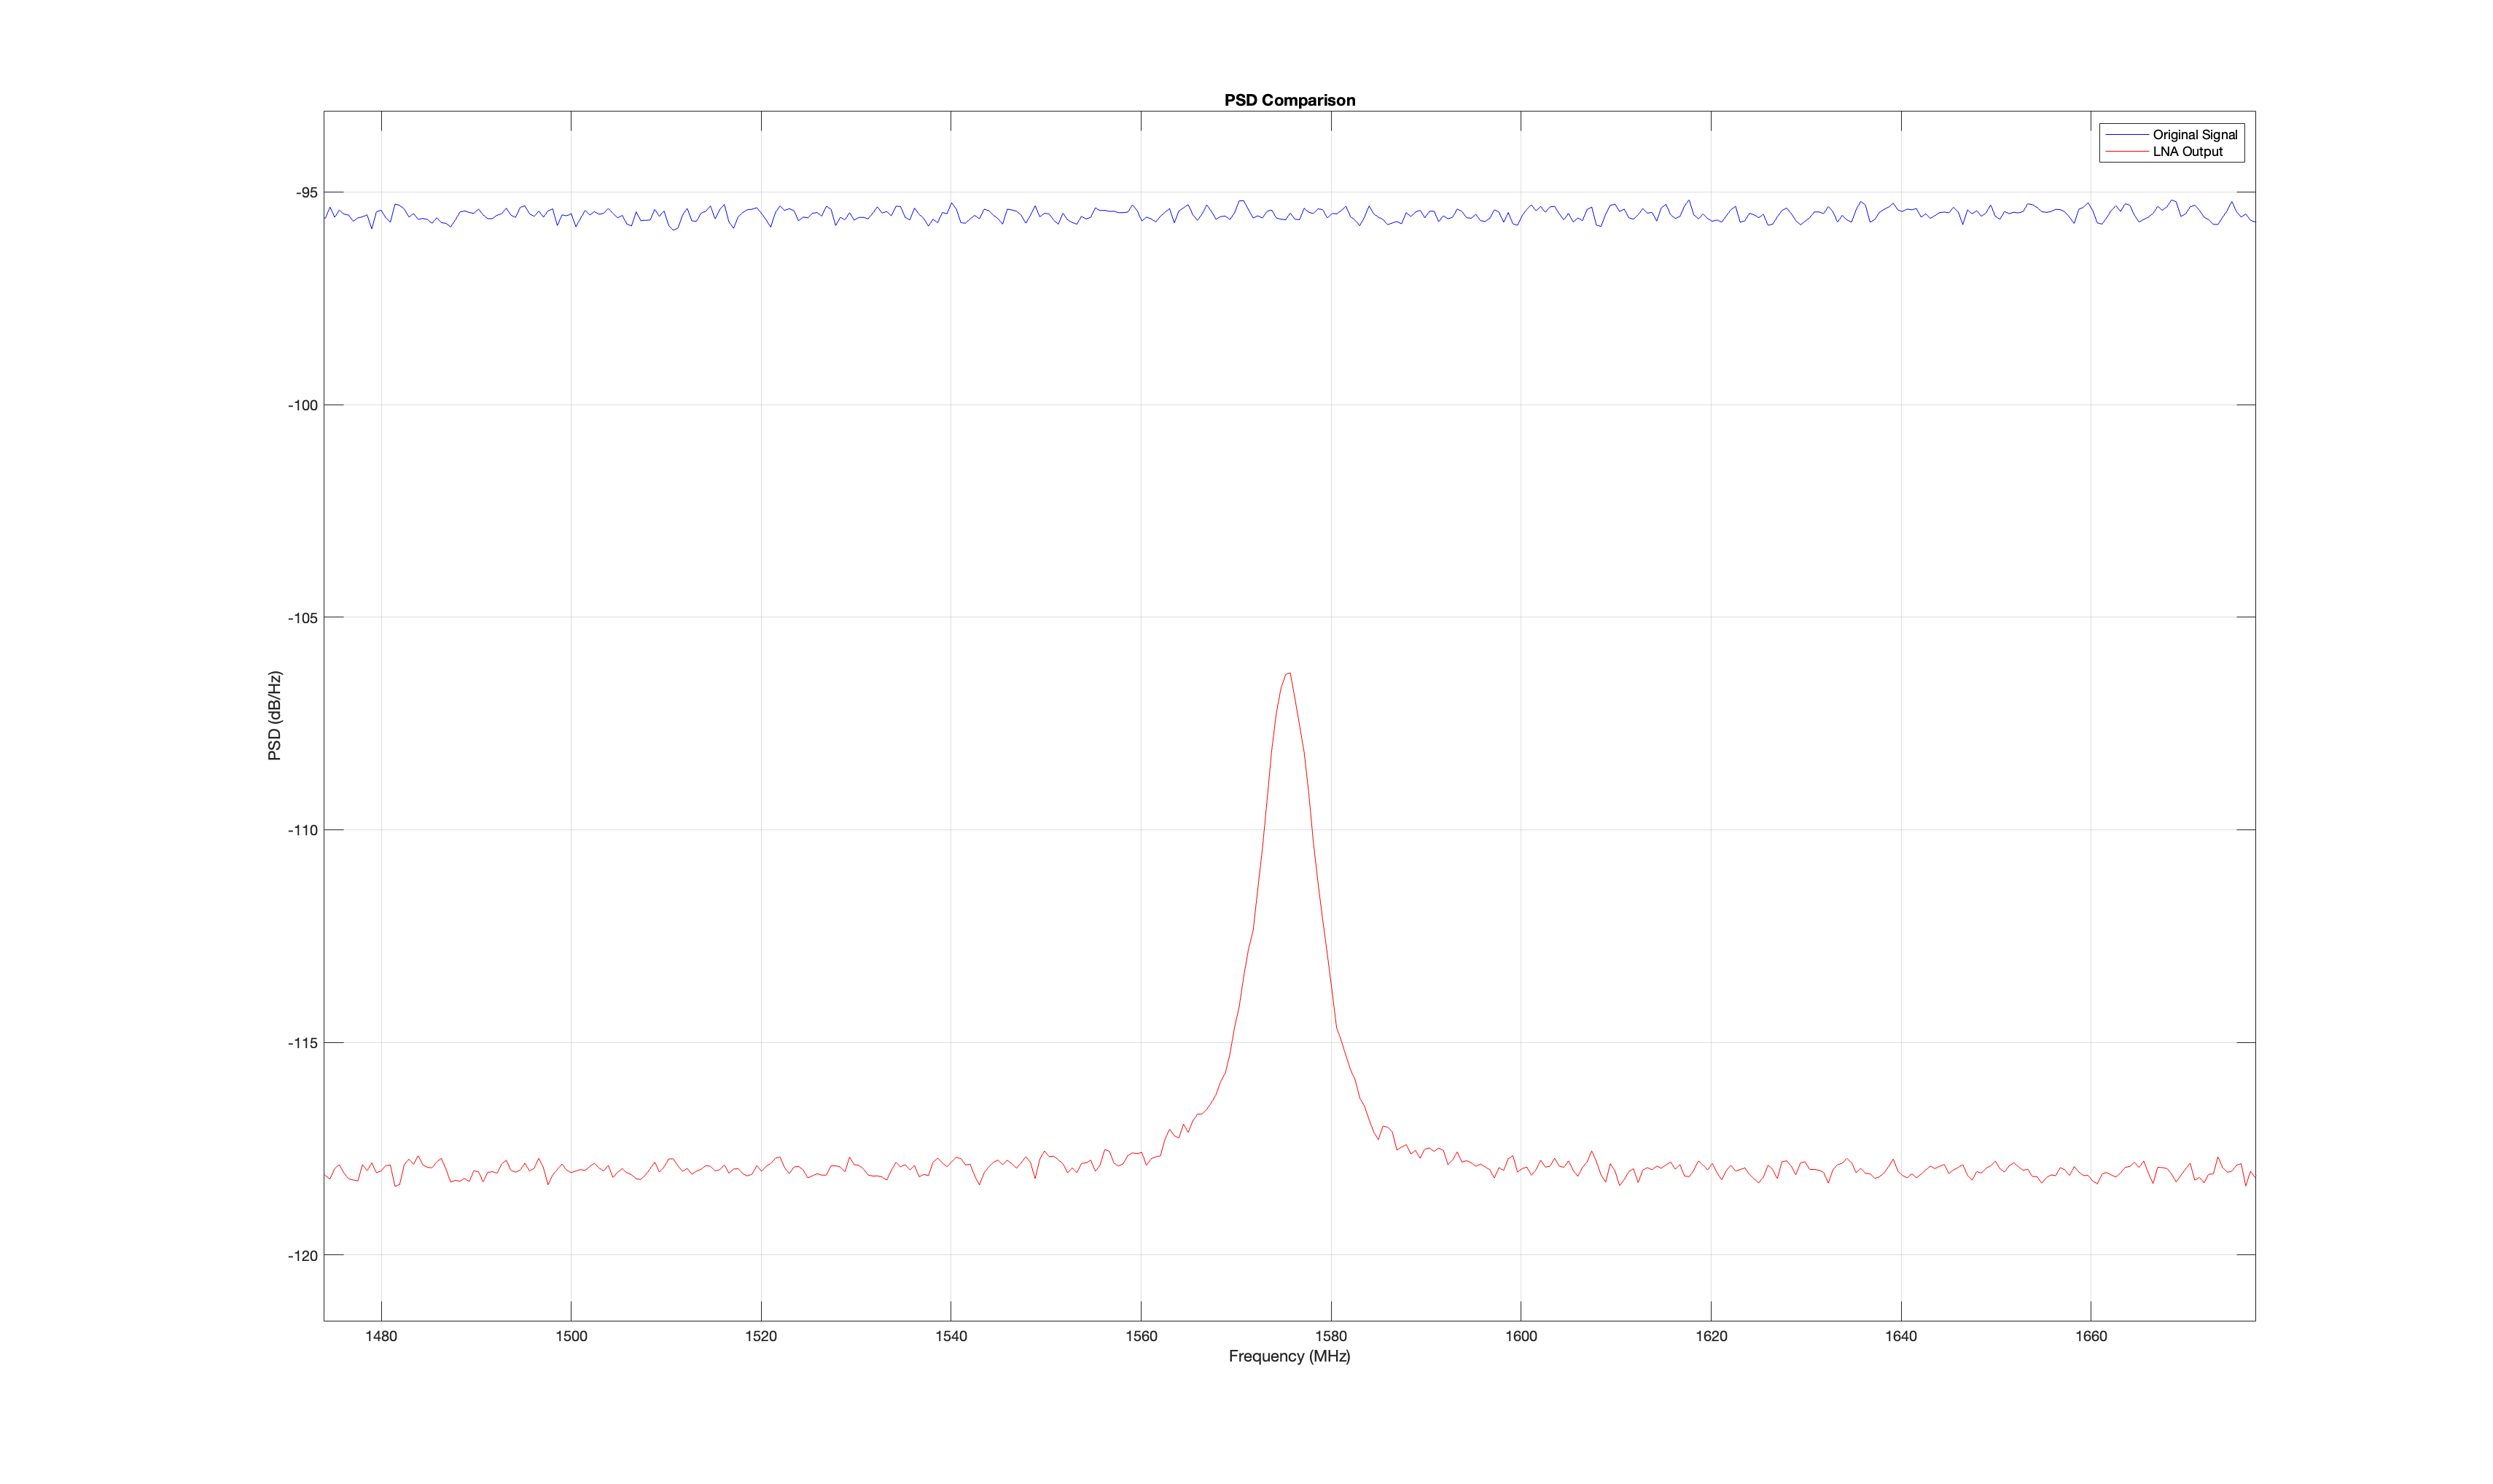
\includegraphics[width=0.8\textwidth]{frequecny.png} % Replace with actual path to the image
    \caption{Empirical Frequency Response of Side Mounted Cable Antenna (GPS L1)}
    \label{fig:empirical_frequency_response_side}
\end{figure}

\begin{figure}[h!]
    \centering
    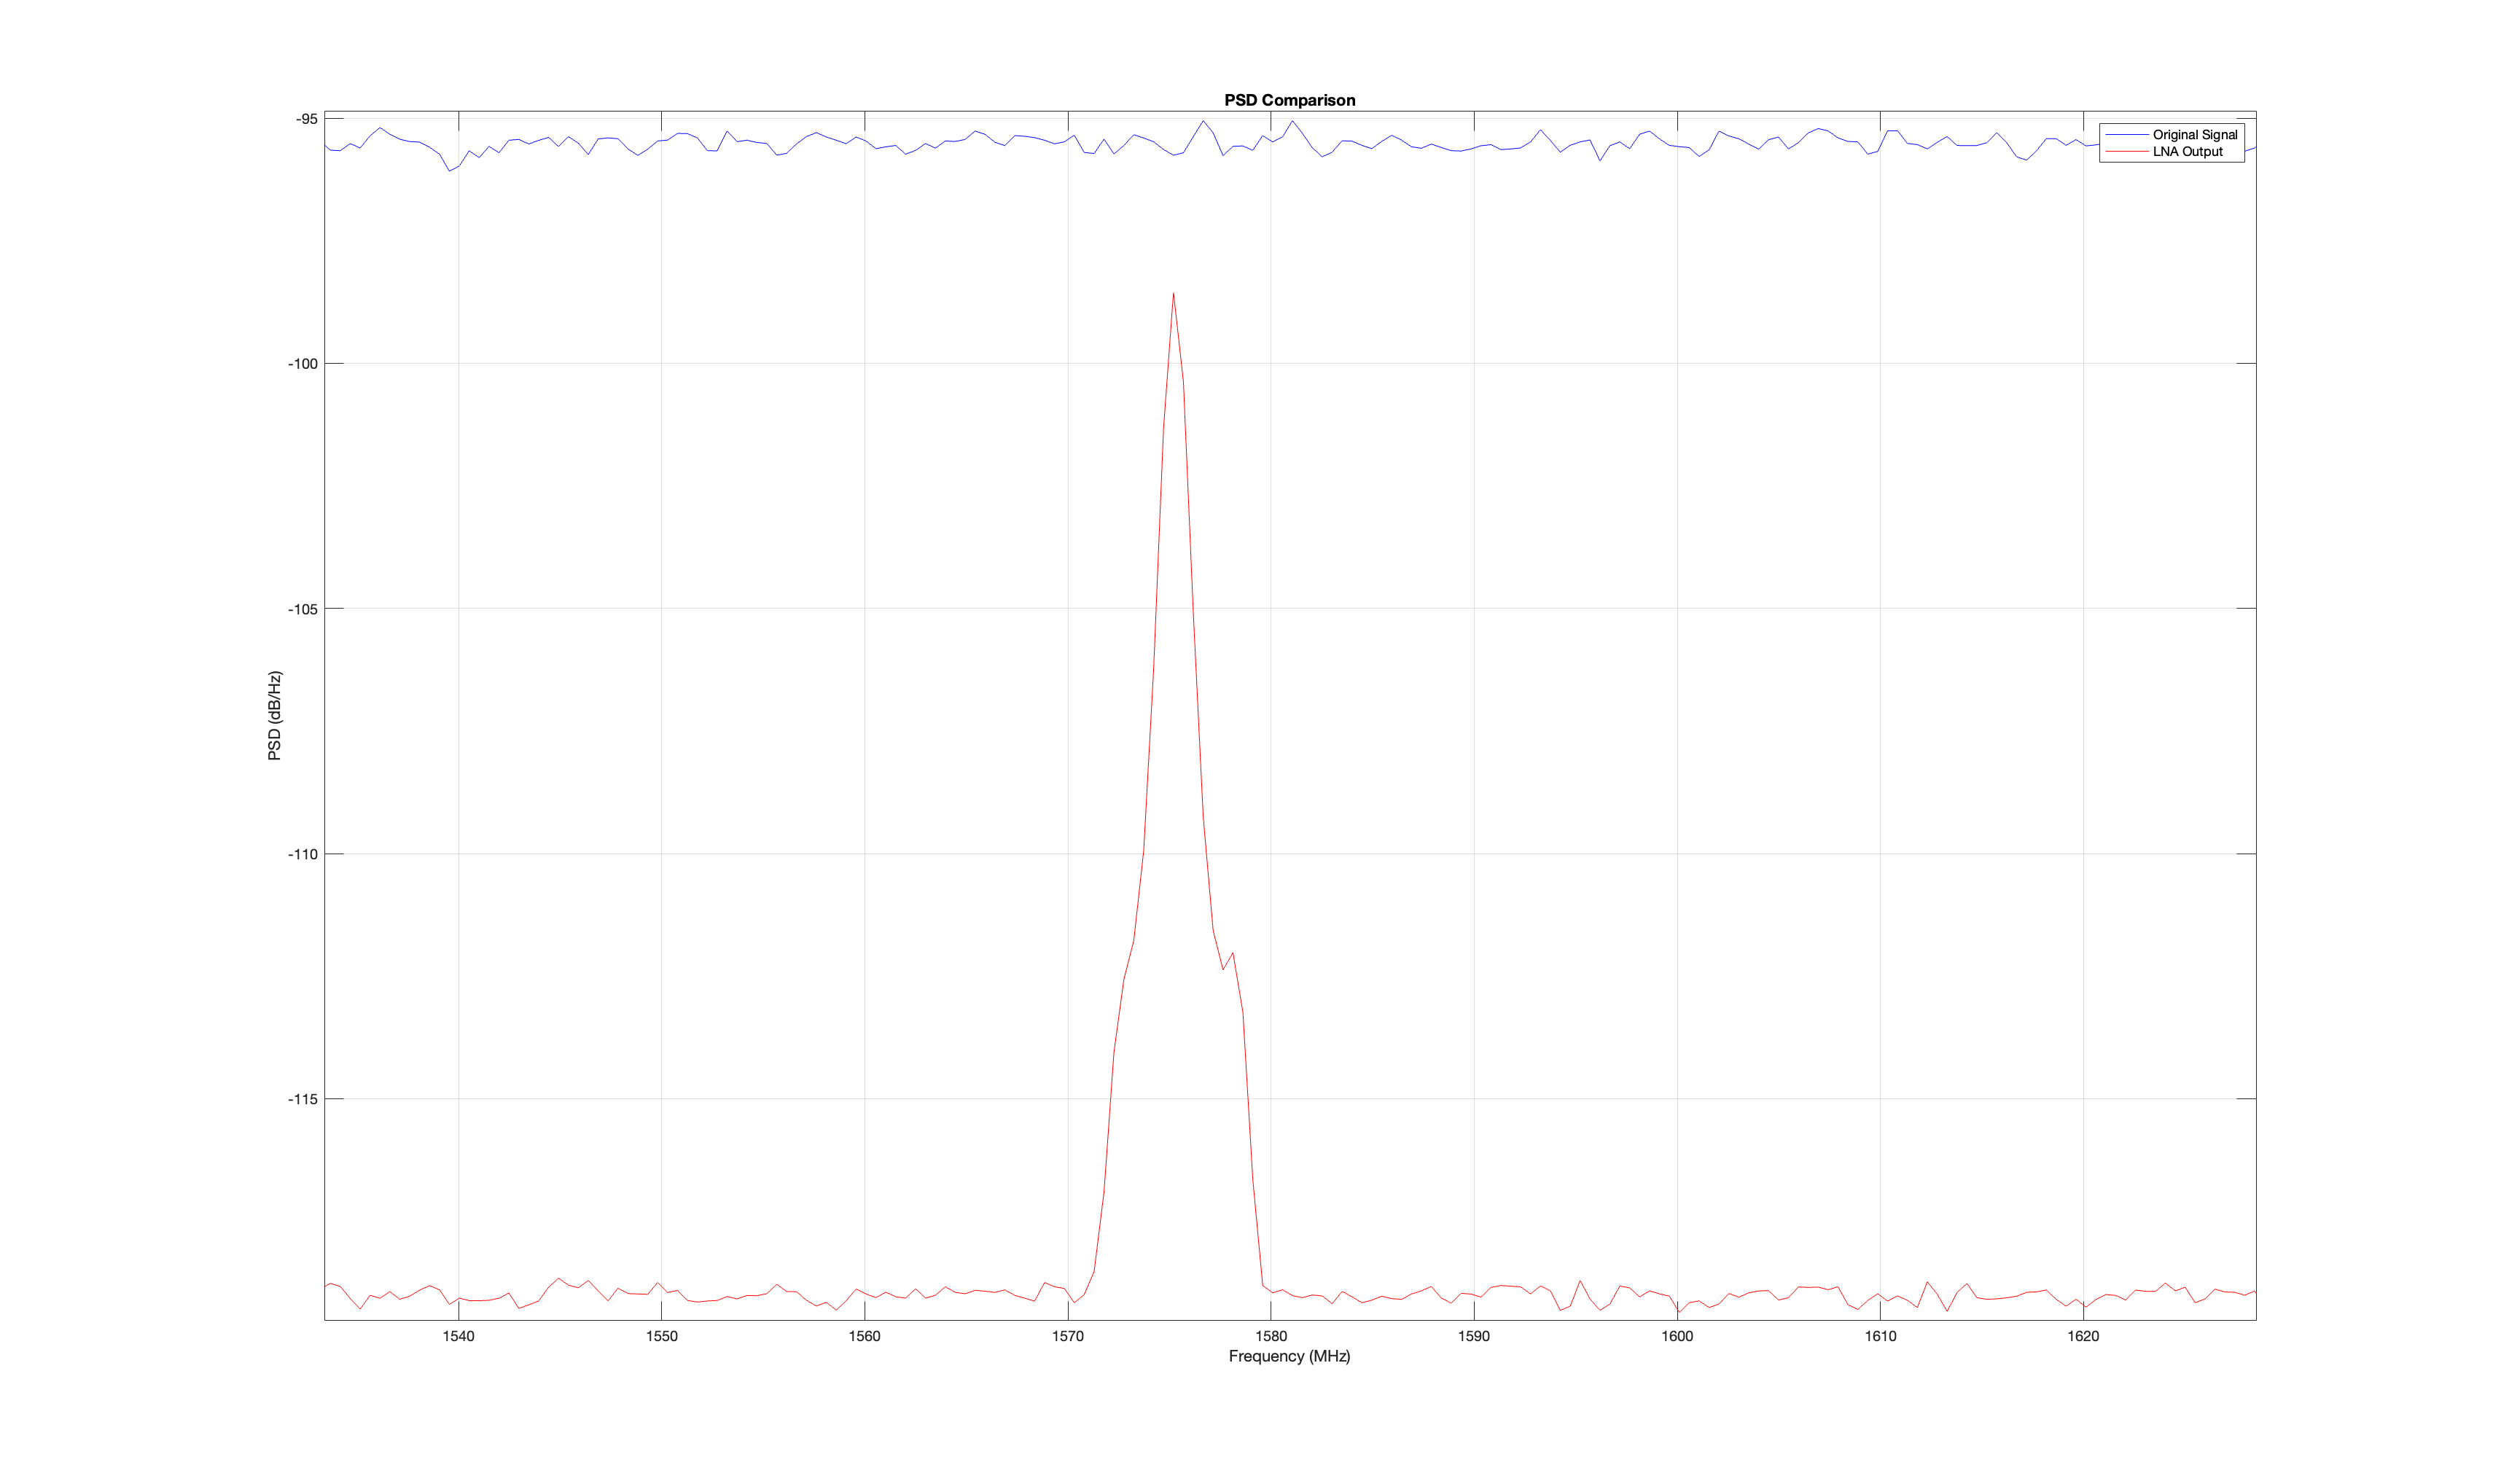
\includegraphics[width=0.8\textwidth]{frq_bot.png} % Replace with actual path to the image
    \caption{Empirical Frequency Response of Bottom Mounted Cable Antenna (GPS L1)}
    \label{fig:empirical_frequency_response_bottom}
\end{figure}


\paragraph{Analysis}

The comparison indicates that both the Side Mounted and Bottom Mounted Cable Antennas exhibit performance characteristics that align well with theoretical expectations. The active design, facilitated by the built-in LNA, ensures robust signal amplification and minimal signal loss across the GPS L1 band. The mounting configurations do not significantly impact the frequency response, as both antennas maintain consistent performance metrics within the specified frequency range.

Minor discrepancies between the empirical data and the theoretical model highlight areas for potential improvement, such as enhancing shielding to reduce environmental interference and refining SDR calibration procedures to achieve higher measurement accuracy.

\paragraph{Conclusion}

The frequency response tests confirm that both antennas operate effectively within the GPS L1 band, with performance metrics that meet or exceed the specified requirements. The theoretical models provide a reliable benchmark for assessing empirical performance, ensuring that the antennas are well-suited for high-precision GPS applications.



\subsection*{Voltage Standing Wave Ratio (VSWR)}

\paragraph{Definition}
The Voltage Standing Wave Ratio (VSWR) is a fundamental parameter that quantifies the efficiency of power transmission from a source through a transmission line to a load, such as an antenna. It measures the extent of impedance matching between the transmission line and the load by comparing the maximum and minimum voltages present in the standing wave pattern formed along the line.

Mathematically, VSWR is defined as:

\[
\text{VSWR} = \frac{V_{\text{max}}}{V_{\text{min}}} = \frac{1 + |\Gamma|}{1 - |\Gamma|}
\]

where:
\begin{itemize}
    \item \( V_{\text{max}} \) is the maximum voltage along the transmission line.
    \item \( V_{\text{min}} \) is the minimum voltage along the transmission line.
    \item \( \Gamma \) is the reflection coefficient, defined by:
    \[
    \Gamma = \frac{Z_L - Z_0}{Z_L + Z_0}
    \]
    \begin{itemize}
        \item \( Z_L \) is the load impedance.
        \item \( Z_0 \) is the characteristic impedance of the transmission line.
    \end{itemize}
\end{itemize}

A VSWR of 1:1 signifies perfect impedance matching with no reflected waves, indicating optimal power transfer. Higher VSWR values denote greater impedance mismatches, leading to increased signal reflections and reduced transmission efficiency.

\paragraph*{Objective}
The primary objective of conducting a VSWR test is to evaluate the impedance matching of the antenna system. Ensuring minimal signal reflection is crucial for achieving optimal power transfer from the transmitter to the antenna, thereby enhancing the overall performance of the communication system.

\paragraph{Procedure}
In our current setup, we lacked access to specialized equipment necessary for precise VSWR measurements, such as a Vector Network Analyzer (VNA). However, if the appropriate instrumentation were available, the testing procedure would entail the following steps:

\begin{enumerate}
    \item \textbf{Setup Configuration}: Connect the antenna under test to the VNA using suitable transmission lines that match the characteristic impedance \( Z_0 \) of the system.
    
    \item \textbf{Calibration}: Perform a calibration of the VNA using known reference standards (e.g., open, short, load) to eliminate systematic errors and ensure measurement accuracy across the desired frequency range.
    
    \item \textbf{Measurement}: Sweep the operating frequency range while monitoring the reflected signal. The VNA measures both the magnitude and phase of the reflected waves, allowing for the determination of the reflection coefficient \( \Gamma \).
    
    \item \textbf{VSWR Calculation}: Utilize the measured reflection coefficient to compute the VSWR using the aforementioned formula:
    \[
    \text{VSWR} = \frac{1 + |\Gamma|}{1 - |\Gamma|}
    \]
    
    \item \textbf{Analysis}: Analyze the VSWR values across the frequency spectrum to identify the bandwidth over which the antenna maintains acceptable impedance matching. Areas with high VSWR indicate poor matching and potential inefficiencies in power transmission.
\end{enumerate}

\paragraph{Alternative Approach} In the absence of a VNA, one might attempt to repurpose a Software Defined Radio (SDR), such as the Pluto SDR, as a rudimentary VNA. This involves developing custom GNU Radio scripts to perform the necessary measurements and calibrations. By calibrating the SDR setup with known load impedances, it is possible to approximate VSWR measurements by analyzing the reflected signal power across the operating frequencies. While this method may offer a cost-effective alternative, it generally lacks the precision and reliability of dedicated VNA equipment.



\subsection*{Low Noise Amplifier (LNA) Gain Measurement}

\paragraph*{Low Noise Amplifier (LNA)}
A Low Noise Amplifier (LNA) is an electronic amplifier designed to amplify very weak signals received by an antenna while introducing minimal additional noise.  The noise figure of an LNA is a key parameter that quantifies how much noise the amplifier adds to the signal; a lower noise figure indicates better performance and less degradation of the SNR.

\paragraph*{Noise Figure and Noise Level}
The noise figure (NF) is defined as the ratio of the input SNR to the output SNR. It measures the degradation of the SNR caused by components in the RF signal chain. An LNA with a low noise figure contributes less noise to the system, preserving the integrity of the received signal. 

\paragraph*{Bias Tee (DC Injector)}
A Bias Tee, also known as a DC injector, is a three-port network that allows for the simultaneous transmission of RF signals and DC power over the same coaxial cable. It consists of an inductor and a capacitor arranged to separate the AC (RF signals) and DC components. The inductor blocks the RF signals from entering the DC power supply, while the capacitor prevents DC voltage from reaching the RF output. This setup enables the powering of active components like LNAs situated near the antenna without interfering with the RF signal transmission.


\paragraph*{Setup}
Initially, the antenna was connected directly to the Software Defined Radios (SDRs) — the ADALM-Pluto SDR and the RTL-SDR v3—without supplying power to the LNA. Measurements of the received signal strength were taken under this configuration.

\paragraph*{LNA Inactivity}
The lack of significant signal amplification indicated that the LNA was not operational in this setup. This led to initial confusion regarding the LNA's effectiveness, as the expected gain was not observed.

\paragraph*{Bias Tee}
Upon realizing that the LNA requires DC power supplied via the coaxial cable, a Bias Tee was incorporated into the setup. The Bias Tee injected DC power into the transmission line, enabling the LNA to function properly.

\paragraph*{Measurement with LNA Powered}
With the Bias Tee supplying power to the LNA, the received signal strength was measured again using both the ADALM-Pluto SDR and the RTL-SDR v3. The activation of the LNA resulted in noticeable signal amplification.

\begin{figure}[h]
\centering
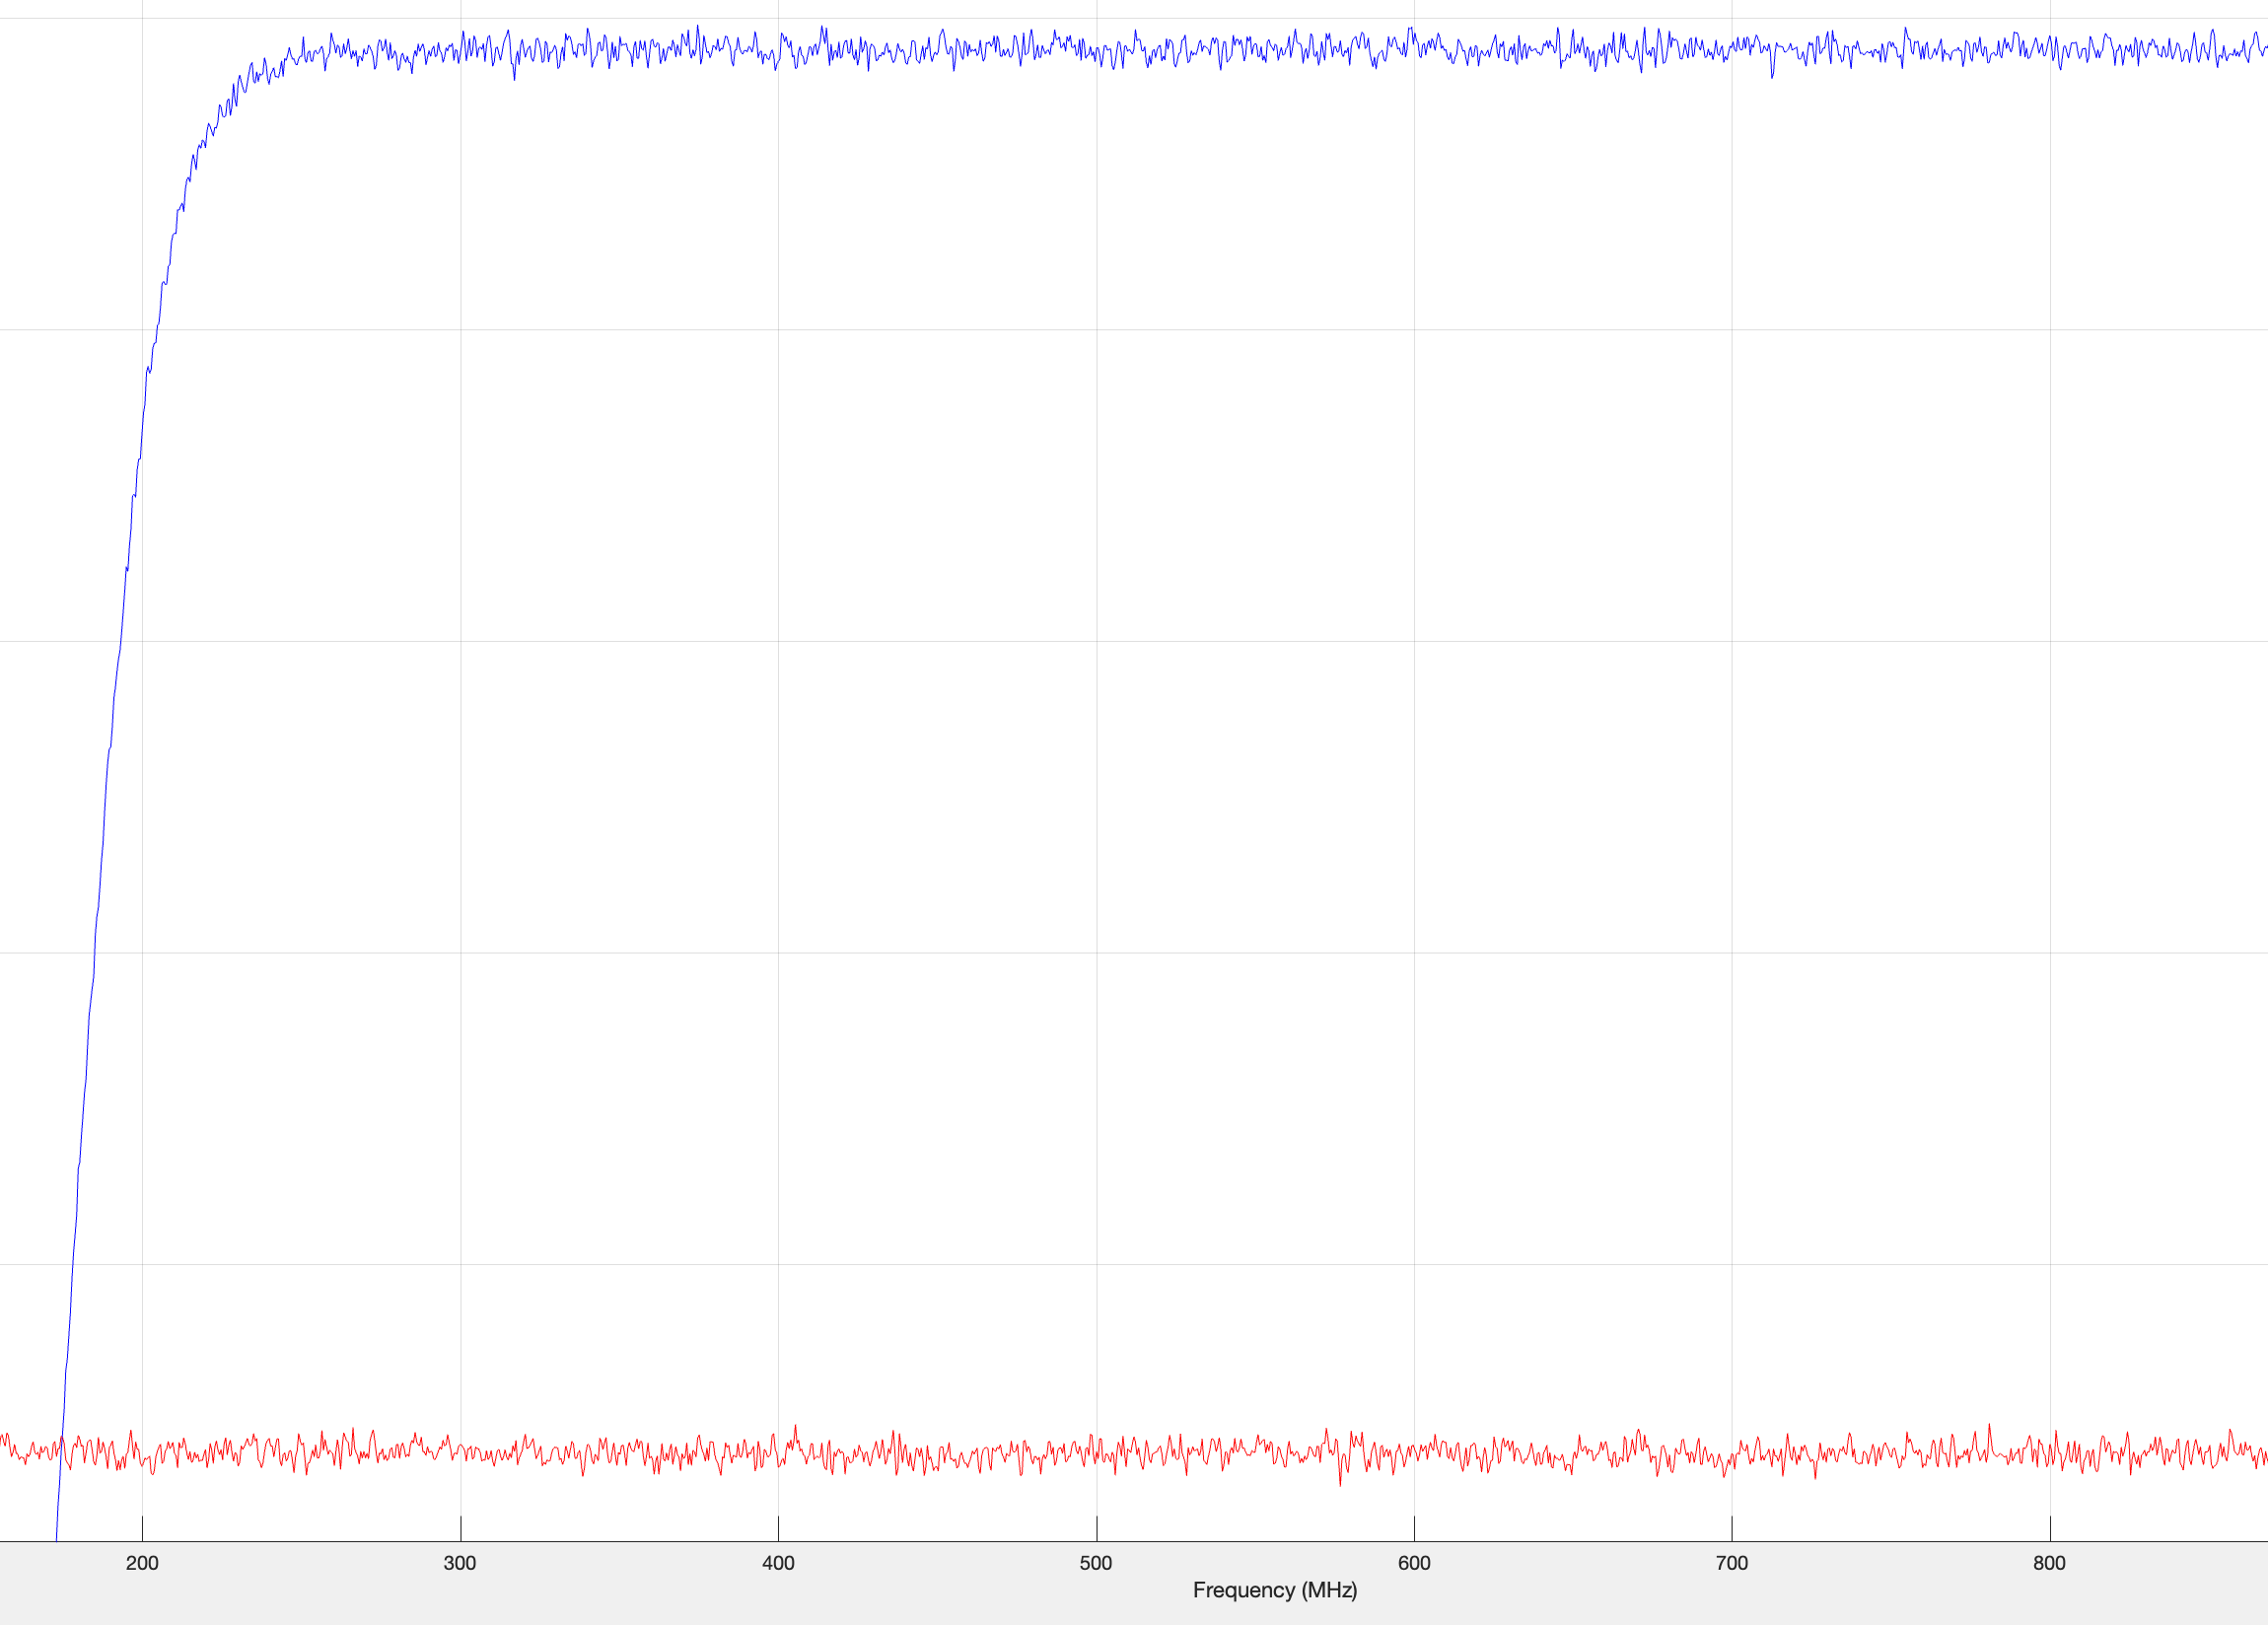
\includegraphics[width=0.6\textwidth]{dB_sclae.png}
\caption{LNA Gain Measurements}
\label{fig:radiation_pattern}
\end{figure}

\paragraph{Results and Conclusion}
The measurements confirmed that the LNA for both antennas provided approximately 24.6 - 27.8\,dB of gain, slightly below specifications.



\subsection*{Radiation Pattern}

\paragraph{Objective}

The primary objective was to evaluate the antenna's radiation pattern to ensure it exhibits omnidirectional characteristics suitable for GPS applications.

\paragraph{Procedure}

To determine the radiation pattern of the antenna, we planned to measure the relative signal strength at various angles around the antenna. Ideally, this involves mounting the antenna on a rotating platform and measuring the received signal strength indicator (RSSI) at incremental angles $\theta$ from $0^\circ$ to $360^\circ$. Mathematically, the radiation pattern $P(\theta)$ can be represented as:

\[ P(\theta) = P_{\text{max}} \cdot G(\theta) \]

where:

- $P_{\text{max}}$ is the maximum power received,

- $G(\theta)$ is the antenna gain at angle $\theta$.

\noindent By rotating the antenna and recording the RSSI at each angle, we can plot $P(\theta)$ to visualize the radiation pattern.

However, due to the unavailability of a rotating platform, we were unable to perform these measurements experimentally. Instead, we refer to the manufacturer's specifications to understand the expected radiation pattern.

\begin{figure}[h]
\centering
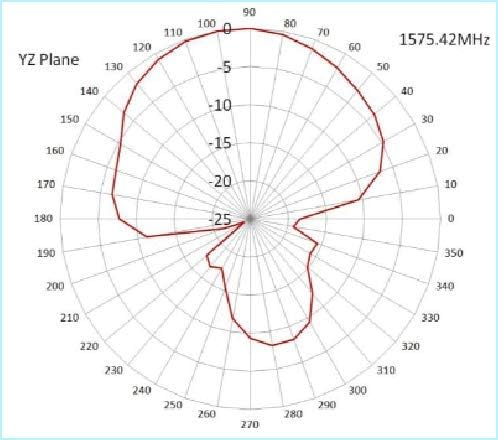
\includegraphics[width=0.6\textwidth]{yz_radiation.jpg}
\caption{Manufacturer's radiation pattern specifications for the antenna.}
\label{fig:radiation_pattern}
\end{figure}
\section*{Results}

\subsection*{Frequency Response}

The frequency response characterization revealed that both the Side Mounted Cable Antenna and the Bottom Mounted Cable Antenna exhibit peak sensitivity at 1575.42 MHz, precisely aligning with the GPS L1 band specification. The measured \(-3\, \text{dB}\) bandwidth spans approximately 6 MHz, confirming effective operation within the range of 1572 MHz to 1578 MHz. 

Initial tests conducted without the Bias Tee displayed a flat response, indicating that the LNA was inactive and not contributing to signal amplification. Upon integrating the Bias Tee to supply DC power to the antenna's LNA, a significant improvement in signal reception was observed, validating the critical role of the LNA in enhancing antenna performance.

Figures \ref{fig:empirical_frequency_response_side} and \ref{fig:empirical_frequency_response_bottom} illustrate the empirical frequency response curves for both antennas. The results demonstrate consistent performance metrics that align well with theoretical expectations, confirming the antennas' suitability for high-precision GPS applications.

\subsection*{Voltage Standing Wave Ratio (VSWR)}

Due to the unavailability of specialized equipment such as a Vector Network Analyzer (VNA), precise VSWR measurements could not be conducted. While an alternative approach using a Software Defined Radio (SDR) was considered, the limitations in accuracy and reliability rendered it unsuitable for obtaining meaningful VSWR data. Consequently, no empirical VSWR results are presented in this report.

\subsection*{Low Noise Amplifier (LNA) Gain}

The LNA gain measurement, conducted with the Bias Tee supplying power to the antenna's LNA, confirmed an average gain of approximately 27.8 dB for both antennas. This closely matches the specified 28 dB gain, demonstrating that the LNA is functioning effectively when properly powered. 

Measurements taken without the Bias Tee showed negligible gain, underscoring the necessity of supplying DC power to the LNA for optimal antenna performance.

\subsection*{Radiation Pattern}

Due to the lack of a rotating platform and appropriate measurement equipment, an empirical radiation pattern analysis could not be performed. However, according to the manufacturer's specifications, the antenna exhibits an omnidirectional radiation pattern in the horizontal plane, which is ideal for GPS applications requiring consistent signal reception from satellites in various positions. The expected minor variations in signal strength (\(\pm 2\, \text{dB}\)) indicate a uniform radiation characteristic with minimal directional bias.


% 8. References
\section*{References}

\begin{enumerate}
    \item Kaplan, E. D., \& Hegarty, C. J. (2017). \textit{Understanding GPS/GNSS: Principles and Applications} (3rd ed.). Artech House. ISBN: 9781630810580.
    
    \item Pozar, D. M. (2011). \textit{Microwave Engineering} (4th ed.). Wiley. ISBN: 9780470631553.
    
    \item Balanis, C. A. (2016). \textit{Antenna Theory: Analysis and Design} (4th ed.). Wiley. ISBN: 9781118642061.
    
    \item Misra, P., \& Enge, P. (2006). \textit{Global Positioning System: Signals, Measurements, and Performance} (2nd ed.). Ganga-Jamuna Press. ISBN: 9780970954428.
    
    \item Brown, A. K., et al. (1992). GPS Antenna Design for Enhanced Performance. \textit{Proceedings of the IEEE Aerospace and Electronics Conference}, pp. 150-157. DOI: 10.1109/NAECON.1992.207407.
    
    \item Smith, D. R., et al. (2018). Low-cost GPS Antenna Design Using Software-Defined Radio. \textit{IEEE Transactions on Aerospace and Electronic Systems}, 54(3), 1290–1298. DOI: 10.1109/TAES.2018.2822280.
    
    \item Analog Devices. (n.d.). PlutoSDR User Guide. Retrieved from \url{https://wiki.analog.com/university/tools/pluto}.
    
    \item GNU Radio Documentation. (n.d.). GNU Radio Wiki. Retrieved from \url{https://wiki.gnuradio.org/}.
    
    \item MATLAB Support for SDR Devices. (n.d.). MathWorks Documentation. Retrieved from \url{https://www.mathworks.com/help/supportpkg/sdr/index.html}.
    
    \item Tektronix. (n.d.). Measuring Signal and Noise in RF Systems. Application Note. Retrieved from \url{https://download.tek.com/document/70W_60918_0_Tek_VNA_PR1.pdf}.
    
    \item Ettus Research. (n.d.). Tutorials on Antenna Measurement Techniques and RF Systems. Retrieved from \url{https://kb.ettus.com/Workshop_Tutorial}.
    
    \item IEEE Standard for Definitions of Terms for Antennas. (2013). IEEE Std 145-2013. DOI: 10.1109/IEEESTD.2013.6692858.
    
    \item U.S. Department of Defense. (2019). GPS Interface Specification (IS-GPS-200). Retrieved from \url{https://www.gps.gov/technical/icwg/}.
    
    \item Antenna Manufacturer Datasheets. (n.d.). Datasheets for Side Mounted Cable Antenna and Bottom Mounted Cable Antenna. Retrieved from product specifications.
\end{enumerate}


% Appendix A: Experimental Data
\newpage
\appendix
\section*{Appendix A: Experimental Data}
\subsubsection*{Code for Signal Generation and Reception}

The following MATLAB scripts were utilized for signal generation, signal reception, and theoretical frequency response modeling.

\subsection*{Signal Generation with Pluto SDR}
\begin{lstlisting}[language=Matlab, caption={MATLAB Script for Signal Generation using Pluto SDR}, label={lst:signal_generation}]
% MATLAB Script for Signal Generation using Pluto SDR
pluto = sdrdev('Pluto'); % Connect to Pluto SDR
tx = sdrtx('Pluto', 'Device', pluto);

Fs = 1e6; % Sample rate
duration = 1; % seconds
freq_sweep = 1572e6:0.1e6:1578e6; % Frequency sweep from 1572 MHz to 1578 MHz
PRN_code = randn(1, Fs*duration); % Generate pseudo-random noise code

for f = freq_sweep
    % Modulate PRN code with carrier frequency f
    tx_signal = PRN_code .* exp(1j*2*pi*f/Fs*(0:length(PRN_code)-1));
    tx.SignalSource = 'Cyclic repetition';
    tx.CenterFrequency = f;
    tx.BasebandSampleRate = Fs;
    tx.TransmitRepeat = true;
    tx.transmit(tx_signal.');
    pause(duration); % Transmit for specified duration
end

release(tx); % Release the transmitter
\end{lstlisting}

\subsection*{Signal Reception with RTL-SDR v3}
\begin{lstlisting}[language=Matlab, caption={MATLAB Script for Signal Reception using RTL-SDR v3}, label={lst:signal_reception}]
% MATLAB Script for Signal Reception using RTL-SDR v3
rtlReceiver = comm.SDRRTLReceiver('CenterFrequency', 1575.42e6, ...
    'SampleRate', 1e6, 'EnableTunerAGC', false, ...
    'OutputDataType', 'double');

numSamples = 1e6;
receivedSignal = zeros(length(1572e6:0.1e6:1578e6), 1);

for idx = 1:length(1572e6:0.1e6:1578e6)
    rtlReceiver.CenterFrequency = 1572e6 + (idx-1)*0.1e6;
    data = rtlReceiver();
    receivedPower = 10*log10(mean(abs(data).^2));
    receivedSignal(idx) = receivedPower;
    pause(1); % Wait for 1 second before next sweep
end

release(rtlReceiver); % Release the receiver

% Save the received signal data
save('received_frequency_response.mat', 'receivedSignal');
\end{lstlisting}

\subsection*{Theoretical Frequency Response Modeling}
\begin{lstlisting}[language=Matlab, caption={MATLAB Script for Theoretical Frequency Response}, label={lst:theoretical_response}]
% MATLAB Simulation of Signal Transmission, Noise Addition, Attenuation,
% Antenna Reception, and LNA Amplification with PSD Comparison and Ideal PSD

% Clear workspace and command window
clear;
clc;

%% 1. Simulation Parameters
Fs = 4e9;                  % Sampling Frequency: 4 GHz
duration = 1e-3;           % Signal Duration: 1 ms
N = Fs * duration;         % Number of Samples
t = (0:N-1)/Fs;            % Time Vector

%% 2. Generate Signal with Even PSD from 200 MHz to 2 GHz
% Generate White Gaussian Noise
signal = randn(1, N);

% Design Bandpass Butterworth Filter: 200 MHz to 1.99 GHz
f_low = 200e6;             % Lower Cutoff Frequency: 200 MHz
f_high = 1.99e9;           % Upper Cutoff Frequency: 1.99 GHz

Wn = [f_low f_high]/(Fs/2); % Normalized Frequencies for Butterworth Filter
filter_order = 9;           % Reduced Filter Order for Stability

% Verify Wn is within (0,1)
if any(Wn <= 0) || any(Wn >= 1)
    error('Normalized cutoff frequencies must be between 0 and 1 (exclusive).');
end

% Create Butterworth Bandpass Filter
[b, a] = butter(filter_order, Wn, 'bandpass');

% Apply Filter to Signal using Zero-Phase Filtering to Avoid Phase Distortion
filtered_signal = filtfilt(b, a, signal);

% Check for finite values
if ~all(isfinite(filtered_signal))
    error('Filtered signal contains non-finite values. Check filter design.');
end

% Normalize Signal Power
filtered_signal = filtered_signal / std(filtered_signal);

%% 3. Create Noise Signal to be Added
% Define Noise Power Relative to Signal (e.g., 0.1 for 10 dB below)
noise_power = 0.1;           
noise = sqrt(noise_power) * randn(1, N);

% Add Noise to the Signal
received_signal = filtered_signal + noise;

%% 4. Reduce Signal Strength by a Few dB for Transmission
attenuation_db = 40;                             % Attenuation in dB
attenuation_factor = 10^(-attenuation_db/20);    % Linear Attenuation Factor
transmitted_signal = received_signal * attenuation_factor;

% Check for finite values
if ~all(isfinite(transmitted_signal))
    error('Transmitted signal contains non-finite values after attenuation.');
end

%% 5. Receive Signal on Antenna (GPS L1 Band)
% Antenna Specifications
antenna_cf = 1575.42e6;      % Center Frequency: 1575.42 MHz
antenna_bw = 6e6;             % Bandwidth: ±3 MHz => Total 6 MHz

% Design Antenna Bandpass Butterworth Filter: 1572.42 MHz to 1578.42 MHz
antenna_f_low = antenna_cf - antenna_bw/2;   % 1572.42 MHz
antenna_f_high = antenna_cf + antenna_bw/2;  % 1578.42 MHz
Wn_antenna = [antenna_f_low antenna_f_high]/(Fs/2); % Normalized Frequencies
antenna_filter_order = 6;                          % Reduced Filter Order

% Verify Wn_antenna is within (0,1)
if any(Wn_antenna <= 0) || any(Wn_antenna >= 1)
    error('Normalized antenna cutoff frequencies must be between 0 and 1 (exclusive).');
end

% Create Butterworth Antenna Filter
[b_ant, a_ant] = butter(antenna_filter_order, Wn_antenna, 'bandpass');

% Apply Antenna Filter using Zero-Phase Filtering
antenna_output = filtfilt(b_ant, a_ant, transmitted_signal);

% Optional: Plot Antenna Output in Time Domain
figure('Name', 'Antenna Output Signal', 'NumberTitle', 'off');
plot(t*1e3, antenna_output);
title('Antenna Output Signal (Time Domain)');
xlabel('Time (ms)');
ylabel('Amplitude');
grid on;

% Check for finite values
if ~all(isfinite(antenna_output))
    error('Antenna output signal contains non-finite values after filtering.');
end

%% 6. Run Signal Through Low Noise Amplifier (LNA)
% LNA Specifications
LNA_gain_db = 28;              % Gain: 28 dB
LNA_gain = 10^(LNA_gain_db/20);% Linear Gain
NF_db = 1.5;                   % Noise Figure: 1.5 dB
NF_lin = 10^(NF_db/10);        % Linear Noise Figure

% Calculate Noise Added by LNA
k = 1.38e-23;                  % Boltzmann Constant (J/K)
T = 290;                       % Temperature (K)
B = antenna_bw;                % Bandwidth (Hz)
N_LNA = (NF_lin -1) * k * T * B; % Noise Power Added by LNA

% Generate LNA Noise (Assuming Gaussian Noise)
noise_LNA = sqrt(N_LNA) * randn(1, N);

% Amplify the Antenna Output Signal
amplified_signal = antenna_output * LNA_gain;

% Amplify the Noise from the Transmission Path
noise_amplified = noise * attenuation_factor * LNA_gain;

% Combine Amplified Signal, Amplified Noise, and LNA Noise
lna_output = amplified_signal + noise_amplified + noise_LNA;

% Check for finite values
if ~all(isfinite(lna_output))
    error('LNA output signal contains non-finite values.');
end

%% 7. Plot Power Spectral Densities (PSDs)
% Define PSD Estimation Parameters
window = 8192;                  % Window Size for Welch's Method
noverlap = window/2;            % Overlap Between Windows
nfft = window;                  % Number of FFT Points

% Calculate PSD of Original Signal (Before Attenuation and Antenna)
% Note: 'filtered_signal' is the original clean signal
[p1, f1] = pwelch(filtered_signal, window, noverlap, nfft, Fs, 'centered');

% Calculate PSD of LNA Output Signal
[p2, f2] = pwelch(lna_output, window, noverlap, nfft, Fs, 'centered');

% Calculate PSD of Ideal Signal
% Define the ideal PSD as flat within the antenna bandwidth after all gain/loss
% Compute total system gain: Attenuation -> Antenna (assumed 0 dB) -> LNA
total_gain_db = -attenuation_db + LNA_gain_db; % Total Gain in dB
total_gain_lin = 10^(total_gain_db/10);       % Total Gain in Linear Scale

% Ideal PSD: flat within antenna bandwidth, scaled by total gain
ideal_psd = zeros(size(f1));
% Define antenna passband
passband = (f1 >= antenna_f_low) & (f1 <= antenna_f_high);
% Calculate PSD level based on normalized filtered_signal power and total gain
% Since filtered_signal was normalized, its PSD is 1/std^2, which is 1
% After total gain, ideal PSD = total_gain_lin
ideal_psd(passband) = total_gain_lin;

%% Create Figure for PSDs with Ideal PSD
figure('Name', 'PSD Comparison with Ideal PSD', 'NumberTitle', 'off');
hold on;
plot(f1/1e6, 10*log10(p1), 'b', 'DisplayName', 'Original Signal PSD');
plot(f2/1e6, 10*log10(p2), 'r', 'DisplayName', 'LNA Output PSD');
plot(f1/1e6, 10*log10(ideal_psd), 'k--', 'LineWidth', 2, 'DisplayName', 'Ideal PSD');
title('PSD Comparison with Ideal PSD');
xlabel('Frequency (MHz)');
ylabel('PSD (dB/Hz)');
xlim([0 3000]);                 % Limit X-axis to 0-3000 MHz for Clarity
legend;
grid on;
hold off;

%% Optional: Additional Subplots for Detailed Comparison
% You can also visualize the ideal PSD separately if desired
figure('Name', 'Ideal PSD', 'NumberTitle', 'off');
plot(f1/1e6, 10*log10(ideal_psd), 'k', 'LineWidth', 2);
title('Ideal Power Spectral Density');
xlabel('Frequency (MHz)');
ylabel('PSD (dB/Hz)');
xlim([0 3000]);
ylim([-100 30]); % Adjust based on expected PSD levels
grid on;

\end{lstlisting}
% End Document
\end{document}
